\graphicspath{{figures/design/}}
\chapter{Test Journal: Potentiometer}\label{appendix:PotMeterTest}
\begin{table}[!h]
\begin{tabular}{l l}
\textbf{Test participants:} & Mathias  \\
\textbf{Date:}  & 20/04-2017
\end{tabular}
\end{table}

\section*{Purpose}
The purpose of the test is to find the angle which corresponds to the voltages of the potentiometers. This will be done for both the arm potentiometer and stick potentiometer.
\section*{Test equipment and components}
\begin{table}[htbp]
	\centering
	\caption{List of measurement equipment and components}\label{tab_appendix:PotMeterMaterial}
	\begin{tabularx}{\textwidth}{lXXXX}
		Name & Brand & Model & AAU-number \\ \toprule
		Multimeter	& Fluke & 37 & 08181 	\\ \rowcolor{lightGrey}
		Oscilloscope	& Agilent & 54621D & 33941 	\\
		Power supply	& Agilent & E3631A & 78577\\ 
		\rowcolor{lightGrey}	
		DC motor & Alsthom BBC & F9M2& 08339\\
		Potentiometer & Bourns & Linear 100 k$\Omega$\newline 0,5\% linearity&\\ 		\rowcolor{lightGrey}
		Potentiometer & Bourns & Linear 100 k$\Omega$\newline 1\% linearity&\\
		Protractor & & &\\ \rowcolor{lightGrey}
		Spirit level & & &
	\end{tabularx}
\end{table}
\section*{Setup}
Measurement setup is seen on \autoref{fig:DCSetup} \
\begin{figure} [htbp]
\hspace*{-3.7cm}  
\centering
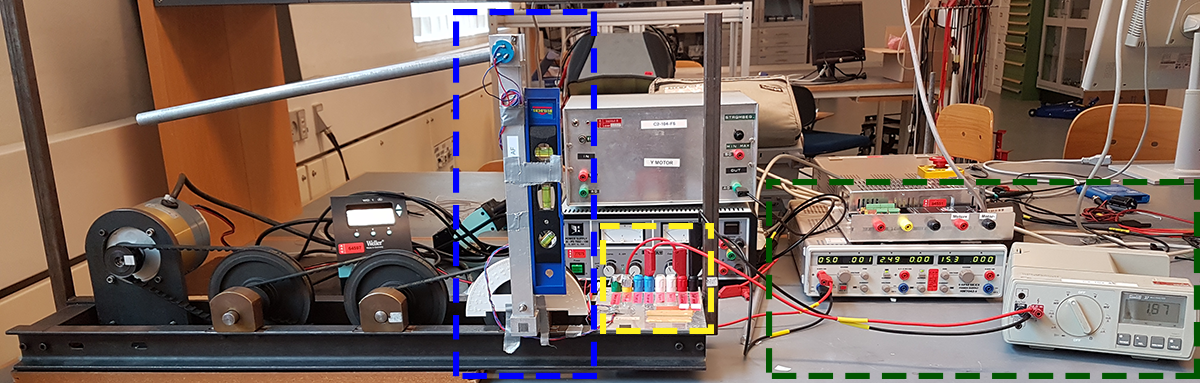
\includegraphics[width=0.95\paperwidth]{figures/appendix/Motor&GearTests/PotMeterSetup}
\caption{Measurement setup.}
\label{fig:DCSetup}
\end{figure}


\startexplain
\explain{\textbf{Blue box} contains the arm, with protractor and spirit level tool. The potentiometer is placed on the back of the opposite site of the arm axis.}{}
\explain{\textbf{Green box} contains the power supply and voltmeter.}{}
\explain{\textbf{Yellow box} contains the power inputs and sensor outputs.}{}
\stopexplain

\section*{Method}
The procedure for the test is as following:
\begin{enumerate}
\item Supply the sensor with 5 V and ground trough the input and output connection board in the yellow box. 
\item Attached the potentiometer of the arm to the voltmeter, the stick is not considered during measurement of the arm.
\item Use the spirit level to place the arm in vertical position which is the systems 0$^\circ$ 
\end{enumerate}
\section*{Raw data}
\begin{table}[htbp]
\centering
\begin{tabular}{lll}
\hline
Position ($^\circ$) & Voltage Pot$_{arm}$ (V) & Voltage Pot$_{stick}$ (V) \\ \hline
-90$^\circ$         & 0,437 V                 & 1,209 V                   \\
-45$^\circ$         & 1,146 V                 & 1,910 V                   \\
0$^\circ$           & 1,860 V                 & 2,610 V                   \\
45$^\circ$          & 2,573 V                 & 3,315 V                   \\
90$^\circ$          & 3,270 V                 & 4,060 V                   
\end{tabular}
\caption{Angle position and corresponding voltage.}
\label{AngleTable}
\end{table}
\section*{Data processing}
\section*{Conclusion}


